\documentclass[11pt]{article}
\usepackage{xltxtra}
\usepackage{unicode-math}
\usepackage{listings}
\usepackage{color}
\definecolor{codegreen}{rgb}{0,0.6,0}
\definecolor{codegray}{rgb}{0.5,0.5,0.5}
\definecolor{codepurple}{rgb}{0.58,0,0.82}
\definecolor{backcolour}{rgb}{0.95,0.95,0.92}
\lstset{language=Python,morekeywords={microbit,button_a,button_b,is_pressed,wait,display,scroll,show,Image,sleep  },columns=flexible,upquote=true,numbers=left,  backgroundcolor=\color{backcolour},   
    commentstyle=\color{codegreen},
    keywordstyle=\color{magenta},
    numberstyle=\tiny\color{codegray},
    stringstyle=\color{codepurple},
    basicstyle=\ttfamily\footnotesize,}


\begin{document}
\setmainfont[Mapping=tex-text,Ligatures=Common]{Arno Pro}
\setsansfont[Mapping=tex-text,Scale=MatchLowercase]{Myriad Pro}
\setmonofont[Mapping=tex-text,Scale=MatchLowercase]{Cascadia Code}
\setmathfont{Asana-Math}

\title{Δέκα απλά προγράμματα με το micro:bit}

\author{}
\date{}
\maketitle
\section{Buzzer}
Σε ένα παιχνίδι με δύο παίκτες ο ένας παίκτης πατάει το κουμπί Α και ο άλλος το κουμπί Β, ποιό κουμπί πατήθηκε πρώτο;

Η λειτουργία του προγράμματος είναι να δείχνει την εικόνα:
\begin{figure}[!h]
\begin{center}
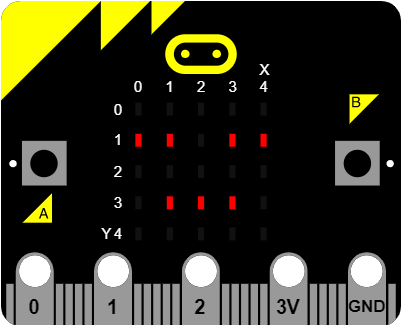
\includegraphics{asleep.png}
\end{center}
\end{figure}

Όταν κάποιος παίκτης πατήσει το δικό του κουμπί εμφανίζεται για 5 δευτερόλεπτα το Α ή το Β αντίστοιχα.
\begin{figure}[!h]
\begin{center}
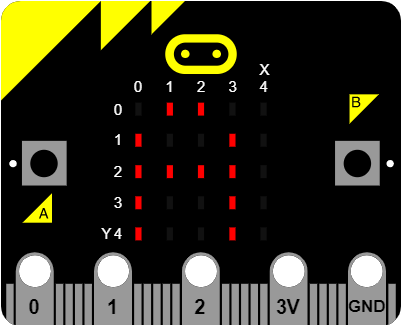
\includegraphics{a.png}\hspace{5em}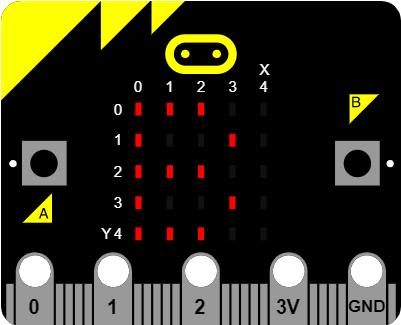
\includegraphics{b.png}
\caption{Image.ASLEEP}
\end{center}
\end{figure}

Το παρακάτω πρόγραμμα υλοποιεί αυτή τη λειτουργία:
\begin{lstlisting}
#buzzer
#show the fastest of two players
from microbit import *

display.scroll('Buzzer', wait = True)

while True:
    display.show(Image.ASLEEP)
    if button_a.is_pressed():
        display.show('A')
        sleep(5000)
    if button_b.is_pressed():
        display.show('B')
        sleep(5000)
\end{lstlisting}

Ο λογική του προγράμματος είναι να δείχνει την εικόνα \lstinline{Image.ASLEEP}, να ελέγχει αν πατήθηκε το Α και στη συνέχεια να ελέγχει αν πατήθηκε το Β. Όταν δεν πατιέται κανένα κουμπί εμφανίζεται η εικόνα \lstinline{Image.ASLEEP}  με την εντολή:
\begin{lstlisting}[firstnumber=8]
display.show(Image.ASLEEP)
\end{lstlisting}
για κάθε ένα από τα κουμπιά το πρόγραμμα ελέγχει αν πατήθηκε και αν πατήθηκε το εμφανίζει με την εντολή \lstinline{display.show}  στη συνέχεια το micro:bit δεν κάνει τίποτα για 5 δευτερόλεπτα που είναι 5000 χιλιοστά του δευτερολέπτου \lstinline{sleep(5000)} ώστε να προλάβουμε να δούμε το Α ή το Β.
\end{document}